
\documentclass[letterpaper, 11 pt, conference]{ieeeconf}  % Comment this line out if you need a4paper


\usepackage{hyperref}
\usepackage{url}
\usepackage[pdftex]{graphicx}
\usepackage{amsfonts}
\usepackage{subfigure} 
\usepackage{algorithm}
%\usepackage{algorithmic}
\usepackage{amsmath}
\usepackage{bm}
\usepackage{algcompatible}
\usepackage{framed}
\usepackage{balance}

\usepackage{graphics} % for pdf, bitmapped graphics files
\usepackage{caption}
\usepackage{epsfig}
\usepackage{wrapfig}
\usepackage{breqn}

\DeclareMathOperator*{\argmax}{arg\,max}

\pdfminorversion=4

\IEEEoverridecommandlockouts                              % This command is only needed if 
                                                          % you want to use the \thanks command
\overrideIEEEmargins                                      % Needed to meet printer requirements.

\author{Wenbo Xu, Wenwen Zhang, Yichi Zhang}

\title{
	EE 382C: Multicore Computing \protect\\
	\Large \bf Parallel GPU based Algorithms for Image Processing
}

\begin{document}
\maketitle
\thispagestyle{empty}
\pagestyle{empty}


\section{Abstract}
  

\section{Introduction}

\section{Gaussian filter}

\section{Optimization}

\subsection{Pageable vs. Pinned Memory}
Host data allocations are pageable by default, which means can be paged in/out between RAM and disk. However, GPU cannot access data directly from pageable memory, but from pinned memory, which means page-locked. Hence, whenever a data transfer is invoked on pageable memory, the CUDA driver has to allocate a temporary pinned memory array to copy host data and then transfer it to the device. \par
\begin{figure}[h]
	\centering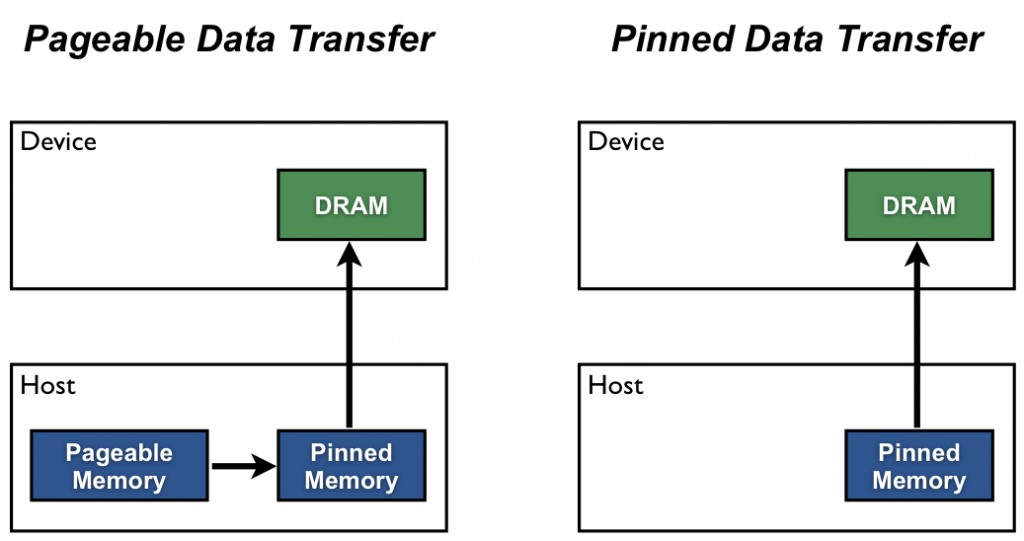
\includegraphics[width=70mm]{pinned.jpg}
	\caption{CUDA data transfer}
	\label{CUDA data transfer.}
	\cite{Mark}
\end{figure}
We can avoid the cost of this overhead by using pinned memory for host instead of pageable memory. In this case, we use \textit{cudaMallocHost()} and \textit{cudaFreeHost()}. Compare to the \textit{malloc()} and \textit{free()}, \textit{cudaMallocHost()} and \textit{cudaFreeHost()} are more expensive with additional overheads. Then, the question has been raised about how should we made the tradeoff. According to figure below, pinned memory is faster when the size of data to be transfered is larger than 16MB. \par
\begin{figure}[h]
 	\centering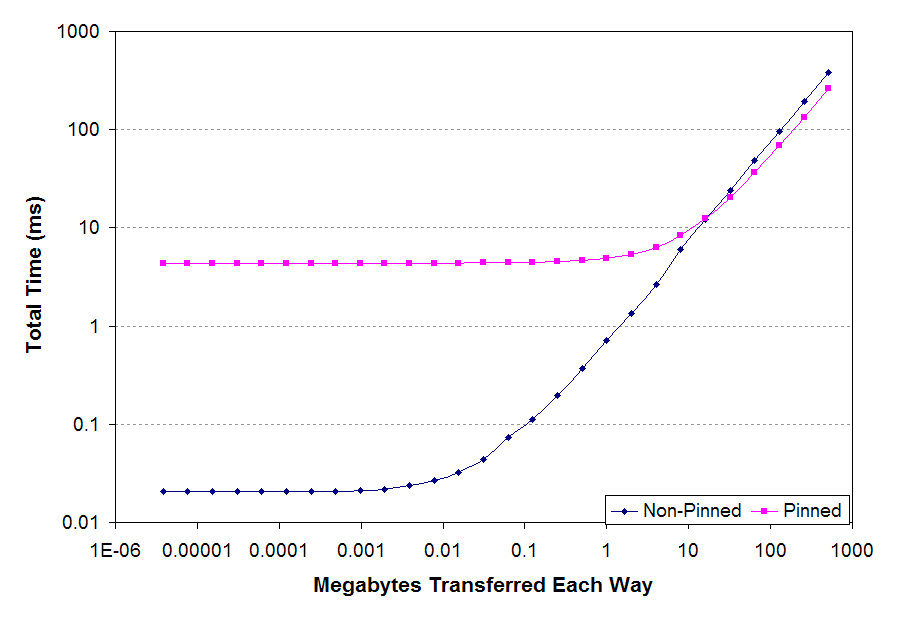
\includegraphics[width=70mm]{pinned_trade_off.png}
 	\caption{Time required to allocate, transfer to the GPU, transfer back to the CPU, and deallocate pinned and non-pinned memory.}
 	\label{Time required to allocate, transfer to the GPU, transfer back to the CPU, and deallocate pinned and non-pinned memory.}
 	\cite{Trade_off}
\end{figure}
This doesn't means we should never use pinned memory when the amount of data to be transfered is less than 16MB. One example is the asynchronous memory copy, \textit{cudaMemcpyAsync()} can be used only with pinned memory. The details of how asynchronous memory copy would be used to improve the efficiency will be discussed in next section.

\subsection{Streams}

\bibliographystyle{abbrv}
\begin{thebibliography}{9}
	\bibitem{Mark} 
Harries, M. (2012, December). How to Optimize Data Transfers in CUDA C/C++. Retrieved from https://devblogs.nvidia.com/parallelforall/how-optimize-data-transfers-cuda-cc/
	
\bibitem{Trade_off} 
Boyer, M. Choosing Between Pinned and Non-Pinned Memory. Retrieved from https://www.cs.virginia.edu/~mwb7w/cuda_support/pinned_tradeoff.html
	
	

\end{thebibliography}

\end{document}
